\chapter{Development}
\label{cap:cap04}

This chapter covers the software switch development. In section \ref{softfeatures}, we give details about the implementation of the most important OpenFlow 1.3 features, in section \ref{OpenSourceDev}, we describe the open source model adopted for the software switch development. 

\section{Software switch implementation}
\label{softfeatures}

Implementation of an OpenFlow switch depends on the platform for which it is designed. OpenFlow hardware implementation on traditional Application Specific Integrated Circuit (ASIC) chips usually suffer from limitations, like small capacity in the total number of flows and not real support for multiple tables. Unlike hardware, software implementations offer greater flexibility in the implementation of OpenFlow features. In environments where high throughput is not the biggest concern, software switches running on commodity servers can be a low cost replacement option for traditional network switches.

The OpenFlow specification describes OpenFlow switches pipeline and the required and optional building blocks. It does not gives low level details about how these components should be implemented. As long as it works how the specification dictates, switch designers are free to use any data structures and algorithms in order to implement OpenFlow. When defining implementation details, we explored the software implementation freedom to meet the requisites defined on section \ref{sec:sec02}. At the same time, we came up with innovative design decisions towards future extensions of the OpenFlow match field support.  

In this section we discuss how we implemented the OpenFlow 1.3 software switch adding several changes to the base switch - using C \footnote{In this chapter there will be two common words: struct and structure. While struct is a C language keyword and structure is a more generic word for a collection of data variables, both will be used to denote a C struct.}, the switch native programming language, and C++ - in order to support all features and keep it as simple as possible. The next subsections describe this new functionalities in the context of the architecture of the software switch presented in chapter \ref{cap:cap03}.

\subsection{Oflib}
\label{sec:sec41}

The software switch architecture Marshaling/Unmarshaling library, presented in section \ref{(un)pack}, is called Oflib. Although already present in the software switch base code, the library underwent several modifications in old messages and grew with the addition of OpenFlow 1.3 messages.

Every OpenFlow message represented by the Oflib has a common header. This header struct contains only one member, which is the message type information. Using the same initial struct for every message struct allows the implementation of two general functions that abstract marshaling and unmarshaling. In the Listing \ref{msgpackunpack}, we show the definition of these functions. Marshaling, also known as packing, is done by \textit{ofl_msg_pack}. By passing a pointer to the struct \textit{ofl_msg_header} for the function, we can check the message type and apply the message respective marshaling function. Unmarshaling, also known as unpacking, is performed by \textit{ofl_msg_unpack}. In this function, the first bytes of the OpenFlow messages, the \textit{buf} parameter, reveal their types. With this information the function calls the proper function to convert the message for the Oflib format.  
\begin{lstlisting}[caption={Oflib: message pack and unpack base functions}, label=msgpackunpack,]
int ofl_msg_pack(struct ofl_msg_header *msg, uint32_t xid, uint8_t **buf, size_t *buf_len, struct ofl_exp *exp);

ofl_err ofl_msg_unpack(uint8_t *buf, size_t buf_len, struct ofl_msg_header **msg, uint32_t *xid, struct ofl_exp *exp);
\end{lstlisting}

Another Oflib task, discussed in the section \ref{(un)pack}, is message error handling. It checks for bad requests from the controller, for example messages with unknown types and wrong sizes are performed by every unpacking function. In case of error, the function returns the OpenFlow error code for the Datapath, which creates an error message and sends it for the controller, through the Communication Channel.

Addition of new OpenFlow messages in the Oflib is a trivial task. Firstly, the developer needs to define a C struct, with \textit{struct ofl_msg_header} as the first member. Then, write a pack and unpack function. Finally, add the new message type for \textit{ofl_msg_pack} and \textit{ofl_msg_unpack}. Listing \ref{rolerequest} illustrates the OpenFlow 1.3 \textit{Role Request}, implemented during our work. 
\pagebreak
\begin{lstlisting}[caption={Oflib message Role request struct and function definition}, label=rolerequest,]
struct ofl_msg_role_request {
	struct ofl_msg_header header; /* Type OFPT_ROLE_REQUEST/OFPT_ROLE_REPLY. */
	uint32_t role;                /* One of OFPCR_ROLE_*. */
	uint64_t generation_id;       /* Master Election Generation Id */
};

static ofl_err
ofl_msg_unpack_role_request(struct ofp_header *src, size_t *len, struct ofl_msg_header **msg)

static int
ofl_msg_pack_role_request(struct ofl_msg_role_request *msg, uint8_t **buf, size_t *buf_len)
};
\end{lstlisting}

Additionally, the Oflib also has printing functions. This is helpful for logging and debugging in the software switch.      

\subsection{OpenFlow Extended Match}
\label{sec:sec42}

When compared to OpenFlow 1.1, in the number of supported match fields, the version 1.3 of the OpenFlow protocol supports nearly twice as much fields as the former version. This growth was only possible due to changes in the match structure specification. A match structure from OpenFlow 1.1 was a fixed number of fields, carrying 88 bits of information in every message carrying a new flow. Match fields not set in the message were sent, adding unnecessary space overhead.   
In order to keep the protocol evolution and to support more fields, the OpenFlow Extended Match (OXM) was introduced by the OpenFlow 1.2 specification. The OXM format is Type-Lenght-Value (TLV) based and replaces the old fixed match structure. A less restricted definition of the match struct adds more flexibility for the insertion of new match fields. Figure \ref{fig:oxmfield} shows an example of how a field is defined by an OXM field and the TLV respective sizes in bits. The Type of a match field is formed by the OXM Class and OXM Field. An OXM class represents a vendor number, where 0x8000 is the basic class for the specification of the match fields. OXM Field defines the match field. In the example, the field number 15 represents the UDP protocol in OpenFlow. The last bit of the Type is left for the Has Mask field, which indicates if the match is masked or not. Finally, the Length field is the value size.
\\
\begin{figure}[H]
\centering
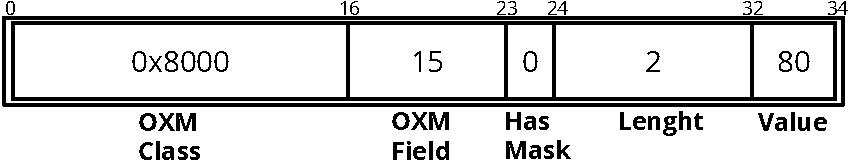
\includegraphics[height=3cm,width=\textwidth,keepaspectratio]{eps/OXMfieldexample.pdf}
\caption{OXM field example}
\label{fig:oxmfield}
\end{figure}

Some challenges arise with the OXM introduction. Whereas extension of match support for messages is solved, there is nothing concerning the packet parsing in the Datapath. The next subsections discuss how our implementation deals with protocol fields extensibility in the software switch. 

    \subsubsection{Packet Parser}
    \label{pktparser}

    Each new protocol added for the OpenFlow specification demands the addition of an specific code to extract the new fields. Distinct protocols may have singular and complex parsing methods. For instance, variable fields such as IP options can require cumbersome deep packet inspection. For this reason, the Packet Parser implementation needs to be flexible and easy to extend. Also, the idea of simple insertion of new match fields meets the ease of extension requisite.    
    
    As a means to achieve a Packet Parser implementation featuring the mentioned characteristics, we have come up with a design which uses a packet description language to assist the parsing. Figure \ref{fig:netbee} shows the Packet Parser model implemented on the switch Datapath. Each module is described as follows:
    
    \begin{figure}[h]
    \centering
    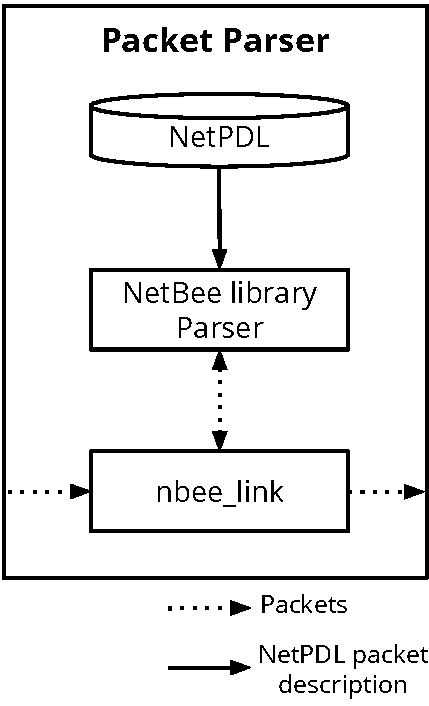
\includegraphics[height=9cm,width=\textwidth,keepaspectratio]{eps/PacketParserEngine.pdf}
    \caption{Packet Parser components}
    \label{fig:netbee}
    \end{figure}
    
    \begin{itemize}
    \item \textbf{NetPDL}. The Network Protocol Description Language (NetPDL)\cite{Risso:2006:NEX:1141112.1141119} is the packet description language. It is a XML-based language and has a large number of protocols and specified encapsulations. In addition, the simple language definition allows easy and fast addition of non available protocol description. An example of how the UDP protocol is described using NetPDL can be foung in the Annex \ref{annex:NetPDLdesc}. In the Figure \ref{fig:netbee} the NetPDL module feeds the parsing library with the description of the OpenFlow 1.3 supported match fields.
    
    \item \textbf{NetBee library Parser}. Netbee is as library for packet processing \cite{nbee}. It is composed by several modules for different types of network application, such as packet filtering and sniffing. For our Packet Parser implementation, we use the Netbee library decoding objects. These objects come from a C++ set of classes and methods that ease packet decoding. To accomplish this, firstly Netbee loads the NetPDL protocols specification into the machine Random Access memory (RAM) and on a packet. Then, received packets are decoded according to the NetPDL description and the extracted information is stored in a protocol tree. Finally, packet field values can be retrieved from the tree using specific methods of the library. 
    
    \item \textbf{nbee_link}. This module is where packets are converted in the flow match structure. Arriving packets are sent for the Netbee library for decoding. From the protocols tree generated by Netbee, the nbee_link module   
extracts the field values and builds the packet match structure that will be sent to the Flow Table look up. The code to extract a protocol is shown by Listing \ref{nbeeparsing}. Using the Netbee method \textit{GetPDMLField}, we get the three ethernet protocol supported fields in OpenFlow 1.3. The second argument of \textit{GetPDMLField} reflects the field name defined in the NetPDL specification. The function \textit{nblink_extract_proto_fields} receives the extracted field value and type and inserts this into the match structure. Another important piece of code is present in the third line. For possible further processing, for instance, the application of a \textit{set field} action, a reference to the protocol position needs to be stored. 
    \pagebreak
    \begin{lstlisting}[caption={Ethernet parsing in the nbee_link module}, label=nbeeparsing,]
    if (protocol_Name.compare("ethernet") == 0 && pkt_proto->eth == NULL)
    {
        pkt_proto->eth = (struct eth_header *) ( (uint8_t*) pktin->data + proto->Position);
        PDMLReader->GetPDMLField(proto->Name, (char*) "dst", proto->FirstField, &field);
        nblink_extract_proto_fields(pktin, field, pktout, OXM_OF_ETH_DST);
        PDMLReader->GetPDMLField(proto->Name, (char*) "src", proto->FirstField, &field);
        nblink_extract_proto_fields(pktin, field, pktout, OXM_OF_ETH_SRC);
        PDMLReader->GetPDMLField(proto->Name, (char*) "type", proto->FirstField, &field);
        nblink_extract_proto_fields(pktin, field, pktout, OXM_OF_ETH_TYPE);
    }
    \end{lstlisting}      
    
    \end{itemize}
    
    An example of how helpful is a flexible design for the Packer Parser is on the support for IPv6 Extension Headers (EH) \cite{rfc2460}. EHs parsing execution is not a trivial task, as there are different types and formats. What is more, IPv6 packets may present complex combinations of headers. In OpenFlow 1.3 support for IPv6 EHs is not based on values, but on a special bitmap that matches in the presence of EHs. Besides, a bit field matches an IPv6 packet only if their EHs are in the recommended order. All of these details would result in a large ammount of code to parse EHs correctly. However, this is done in few lines due to our extensible implementation and the NetPDL language.    
    \subsubsection{Flow Match Prerequisites}
    
    Another change brought by OXMs is the introduction of flow match fields prerequisites. In order to obtain flow match consistency, some match fields require the presence of other fields. For example, matching any ARP protocol field requires the ethertype field having the correct value for an ARP packet. Thereby, inconsistent flows are denied by the Flow Table.  
      
    To map OXM fields prerequisites, a file \footnote{This file was inpired by the old way that OVS handled the Nicira Extended Match (NXM) format. NXM is the format that gave origin to OXM.}, with several C Preprocessor macros, was created. The macros map each field with their respective network layer 2, layer 3 or upper level requisite. In addition there is a field that tells if a field is maskable or not. Listing \ref{oxmrequisite} shows prerequisites and fields macros definition. Also, it gives an example of a field created by the \textit{DEFINE_FIELD} macro. 
\\
\begin{lstlisting}[caption={Ethernet parsing in the nbee_link module}, label=oxmrequisite,]

#define OXM_DL_NONE   (0, 0)
#define OXM_DL_ARP    (ETH_TYPE_ARP, 0)
#define OXM_DL_PBB    (ETH_TYPE_PBB,0)
#define OXM_DL_IP     (ETH_TYPE_IP, 0)
#define OXM_DL_MPLS   (ETH_TYPE_MPLS, ETH_TYPE_MPLS_MCAST)
#define OXM_DL_IPV6   (ETH_TYPE_IPV6, 0)
#define OXM_DL_IP_ANY (ETH_TYPE_IP, ETH_TYPE_IPV6)

#define DEFINE_FIELD_M(HEADER,  DL_TYPES, NW_PROTO, MASKABLE)  \
    DEFINE_FIELD(HEADER,  DL_TYPES, NW_PROTO, MASKABLE)        \
    DEFINE_FIELD(HEADER##_W, DL_TYPES, NW_PROTO, true)

DEFINE_FIELD    (OF_TCP_SRC,        OXM_DL_IP_ANY,   IPPROTO_TCP,    false)

\end{lstlisting}   

    OXMs matches definitions are loaded by the Oflib, and used in the function \textit{oxm_pull_match}, which is called during the match unpack. Among the tests performed to detect invalid OXM fields are: bad prerequisite, duplicate fields, wrongly masked and nonexistent field.  

    \subsubsection{Flow Matching}
    
    In the pursuit for the best way to perform flow matching inside the Flow Table, developers might want to try different algorithms and data structures. For this reason, the switch implements a flexible and easy interface to change the way packets are matched. 
    
    Match fields are part of the software switch \textit{flow_entry} struct. Instead of defining a fixed match as one of the \textit{flow_entry} member, a pointer to Oflib \textit{struct ofl_match_header} is left as a reference for the entry match fields. Therefore, if a developer wants to experiment his own match structure, there is only the need to make it start with an \textit{ ofl_match_header}.    

    This work presents a default flow matching using the Oflib match structure called \textit{ofl_match}. Besides the match header, the struct includes a Hash Map structure to store OXM TLVs. Each OXM entry in the Hash Map has an  exclusive key, created by the combination of the field Type and Length information. Storing only flow specified fields saves memory space, at a small cost of the pointers created to mantain the data structure. Another advantage in the Hash Map use in the match structure is the constant access time for the OXMs. Fast element access is very important for two of the most common operations:
    
    \begin{itemize}
    \item \textbf{Check packet matching}. Packet fields are extracted and matched against the flows. Matching is performed by look ups of the packet fields in the Hash Map.        
    
    \item \textbf{Check flow collision}. Flows collide when a new flow is installed and the Flow Table contains a flow with the same match fields and priority. In this case the old one is replaced by the new one. The Hash Map allows a direct comparison of fields.
    \end{itemize}

    Another detail about flow matching in the software switch is about the linear behavior of Flow Table look up. The Flow Table stores flows in a list ordered by priority. When a packet is sent to the flow match it loops through the flow list until it finds a matching rule or it reaches its end. This is the most simple approach for the flow match and was chosen for its simplicity. Developers who might want to modify the behaviour of Flow Table look up just need to add their own code for the function \textit{flow_table_lookup}.
         
    \subsubsection{Extensible context expression in ’packet-in’}
    
    Former \textit{packet-in} message contained little information about the packet parsed in the Datapath. The only match field present was the switch input port. In order to get the other packet fields, a controller needs to parse the packet header, included in the end of \textit{packet-in}. This causes an unnecessary parsing repetition in the control plane. With the OXM introduction, OpenFlow 1.3 solves this problem sending the extracted packet fields in the form of OXMs, making it easier for the control plane to retrieve the packet fields.  
    
    While an standard switch implementation requires only context information, which are input port, metadata and tunnel_id, our implementation follows the option to add all parsed fields in a \textit{packet-in} message.    

\subsection{Set Field action}
\label{sec:sec43}    

Support for rewriting packet fields exists since the first OpenFlow version. However, it was limited to a small set of fields. In OpenFlow 1.3, with the OXM introduction, a \textit{flow mod} message can carry a  \textit{set field} action with any of the OXMs defined by the specification. It is up for the switch designers to decide which fields are allowed for overwrite.   

Implementation of \textit{set field} is slightly intricate, as the consistence is achieved through the match fields. For instance, a flow with a \textit{set field} action to rewrite the IP source address needs to present in the match fields the same ethertype - 0x800 in hexadecimal - of the IP protocol. The way the pack and unpack of match fields and actions is performed by different functions needs to be checked in the Datapath. When handling a new \textit{flow mod} message, the Flow Table calls the function \textit{dp_actions_check_set_field_req}. This function uses an Oflib function to check if the prerequisites are ok and validates the action.

Another frequent task caused by rewriting fields is protocol CheckSum recalculation. Fields like the IP source and destination, in the case of change, require recalculation of IP and TCP CheckSum values. Fortunately these protocols' CheckSum calculation is very simple \cite{rfc1071}. This is not the case for the SCTP protocol \cite{rfc3309}. SCTP CheckSum is calculated using a Cyclic Redundancy Check (CRC). In order to recalculate the SCTP CheckSum value we used a Python program named pycrc \footnote{pycrc v0.8.2, Available at http://www.tty1.net/pycrc/}. The program takes as input the CRC polynomial and generates all the functions necessary for the calculations. Listings \ref{set_field} shows the code to rewrite the SCTP destination port. In the packet field rewriting we attribute a pointer to the protocol struct representation and to the packet position obtained by the Packet Parser. Doing so, we can easily change the current value of the action value.
\\
\begin{lstlisting}[caption={Ethernet parsing in the nbee_link module}, label=set_field,]
case OXM_OF_SCTP_DST:{
                crc_t crc;
                struct sctp_header *sctp = pkt->handle_std->proto->sctp;                
                size_t len = ((uint8_t*) ofpbuf_tail(pkt->handle_std->pkt->buffer)) - (uint8_t *) sctp;
                uint16_t v = htons(*(uint16_t*) act->field->value);
                sctp->sctp_csum = 0;
                memcpy(&sctp->sctp_dst, &v, OXM_LENGTH(act->field->header));
                crc = crc_init();
                crc = crc_update(crc, (unsigned char*)sctp, len);                            
                crc = crc_finalize(crc);
                sctp->sctp_csum = crc;
                break;        
            }
\end{lstlisting}  

\subsection{Per-flow Metering}

    The Meter Table implementation follows the architectural details and responsibilities of the element described on section \ref{sec:MeterTable}.
Firstly we defined a structure for the Meter Table. The main components are the table features, such as the max number of entries and supported band types, and a Hash Map of meter entries. Other members include a reference pointer to the Datapath, allowing a Meter Table to call the function to send OpenFlow messages; and two counters: one for the number of meter entries and another one for the quantity of bands. Secondly, we implemented a set of functions: initialization and destruction of the Meter Table; \textit{meter mod} and \textit{meter features} messages handlers; find and apply a meter entry.

    Structures of meter entries are composed of a configuration - which contains information about the meter id and meter bands - and a struct for recording statistics. In addition, the meter entry has pointers to the Datapath and the Meter Table, similar to what is done in the Meter Table struct. Finally, it has a list of flow references. If the meter entry is deleted, all flows sending packets to the meter entry are deleted. 

    Meter entry bands are chosen accordingly to a configured rate - in Kilo packets (Kpps) per second or Kilobits per second (Kbps). Thus, it is necessary to measure the flow matched packets in function of one of the specified unities. The first idea to implement rate measuring scheme considered the use of matched flow counters, divided by the number of matched bytes by some time interval. Although easy to implement, this approach proved itself inaccurate after some attempts to limit the bandwidth between two hosts connected to the switch.  
    
    After a better analysis of the task and some literature research, we found and implemented a simple and efficient algorithm used for rate policy: the Token Bucket \cite{Tanenbaum:2002:CN:572404}. Figure \ref{fig:tokenbucket} illustrates how the Token Bucket works within a meter band. Simply put, each meter band has a bucket attached to it. At every second the bucket is refilled with a number of tokens equal to the meter rate. When a packet is sent to the Meter Table, it goes through each band's bucket belonging to the meter entry. Inside the bucket, packets consume a number of tokens equal to their size. If there are enough tokens, the OpenFlow pipeline continues processing the packet, otherwise, the meter band is chosen and executed.               

    \begin{figure}[h]
    \centering
    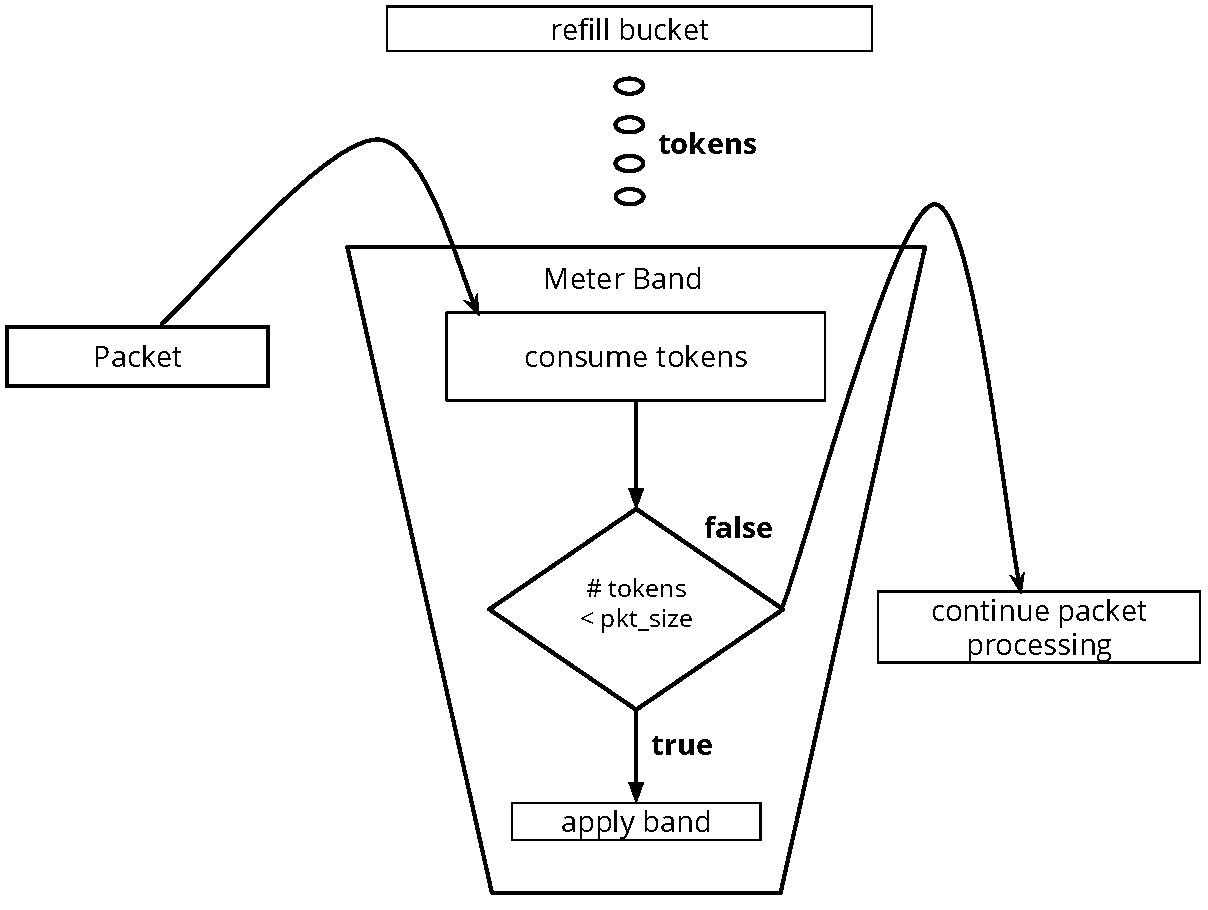
\includegraphics[height=9cm,width=\textwidth,keepaspectratio]{eps/TokenBucket.pdf}
    \caption{Token Bucket Algorithm illustration inside the meter band}
    \label{fig:tokenbucket}
    \end{figure}

\label{sec:sec44}

\subsection{Connection Features}
\label{sec:sec45}

    Network control protocols must be designed with scalability and high availability in mind. Node failures and high traffic loads may cause frustration for early adopters of new technologies, as these two important points are not usually considered by initial versions. Previous OpenFlow versions fall into this category of protocols, often criticized by the lack of mechanisms to handle control plane issues. 
    
    More recent OpenFlow versions try to address control plane scalability and high availability with the addition of new features for OpenFlow connections. Auxiliary connections allow higher scalability for message exchanging, while controller roles try to enable fast failover for OpenFlow controllers. Event filtering, in turn, may be seen as a mechanism that sum up on these two topics. In the next subsections we will see a more detailed description of each feature and how they have been implemented in our software switch.
    
    \subsubsection{Auxiliary Connections}
    
    Auxiliary connections allow a controller to create more than one Communication Channel with a single switch. These connections add the possibility to exploit message parallelism and create a channel for specific types of messages. For instance, a controller can use one connection only for \textit{packet-in} messages. 
    
    As a proof-of-concept we have implemented basic support for auxiliary connections. In our implementation, there is support for only one additional channel and it only carries \textit{packet-in} messages. The following items show steps added in the switch code to handle auxiliary connection.
    
    \begin{itemize}
    \item The software switch sends OpenFlow messages for the Communication Channel, encapsulated into a struct called \textit{ofbuf}. The struct is a buffer that holds information such as the pointer for the first allocated byte and the size of bytes in use. In order to identify which connection is being used to receive or send the message, we have added a new member called \textit{conn_id}. The possible values for \textit{conn_id} are MAIN_CONNECTION and PTIN_CONNECTION.  
    
    \item A new connection listener was added to the Datapath. If an auxiliary connection is specified when running the datapath, the auxiliary listener is opened after the main connection listener.
    
    \item When the Datapath talks to remotes, it searches for the auxiliary connection. If the connection exists, it processes messages received by the connection.
    
    \item On sending OpenFlow messages, the switch by default maps to the MAIN_CONNECTION. If the message is a reply from  a sent message of a sender connection, the connection id is set to the same id used by the sender. In the last case, if the message type is a \textit{packet-in}, the switch uses PTIN_CONNECTION for the connection id. 
    
    \end{itemize}
    
    The start of an auxiliary connection from one controller is disabled by default in our software switch standard program execution. To enable auxiliary connections a user should specify the \textit{multiconn} option in the command line option.   

    \subsubsection{Controller Role}

    Controller Role is a mechanism to permit connection of multiple controllers with different duties. One of the possible use cases of roles is for fast failover, in which when the main controller goes down, a backup controller assumes the switch command. There are three possible roles for controllers: Master, Slave and Equal. A master controller has permissions to send and receive any type of OpenFlow messages. Slaves have very strict default permissions, allowed only to receive a specific set of messages. The last role, Equal, is the default role when a controller connects to the switch and the other controllers connected do not have a defined role.
    
    Role election is totally driven by the control plane, though some additional code is required for the switch. In order to implement controller role support in our software switch we first filtered asynchronous messages received by Slave controllers. Then we restricted slaves to send only read state messages, for example, \textit{flow stats} and \textit{table stats}. The last insertion is the algorithm defined by the specification to handle the \textit{role request} generation_id. Messages with a generation id smaller than previous generation ids seen by the switch are discarded. Listing \ref{rolegenid} presents the function that implements the algorithm.
\pagebreak
\begin{lstlisting}[caption={Ethernet parsing in the nbee_link module}, label=rolegenid,]
static ofl_err
dp_check_generation_id(struct datapath *dp, uint64_t new_gen_id){

    if(dp->generation_id >= 0  && ((uint64_t)(new_gen_id - dp->generation_id) < 0) )
        return ofl_error(OFPET_ROLE_REQUEST_FAILED, OFPRRFC_STALE);
    else dp->generation_id = new_gen_id;
    return 0;
}
\end{lstlisting} 
    \subsubsection{Event Filtering}

    Event Filtering enables controllers to filter undesired asynchronous messages, sent by the switch. Filtering of asynchronous messages is possible for three types: \textit{port status}, \textit{packet-in} and \textit{flow removed}. In addition, a controller can also choose to not receive these message types for the generation reason. For example, a \textit{packet-in} can be generated by an action to output the packet for the controller. This feature, along with auxiliary connections, gives power for controllers to create exclusive message channels.
    
    Message filtering is handled by the Datapath. On a \textit{set async request}, the Datapath sets the controller remote channel with bitmap values sent in the message defined by the OpenFlow 1.3 specification, shown on Listing \ref{asyncmessage}. Each bit set in the bitmap represents a message type and a reason. For instance, a bit with value 4 in \textit{flow_removed_mask[0]}, determines if the controller will receive \textit{flow removed messages} with reason OFPRR_DELETE when the role is Master.  
    
    Filtering happens before the sending of an OpenFlow message. The Datapath function to send an OpenFlow buffer through the Communication Channel checks the remote configuration and the type of message to be sent. If it is one of the three asynchronous messages and the reason and the controller roles matches the remote filtering configuration, the message is dropped. 
    
\begin{lstlisting}[caption={Ethernet parsing in the nbee_link module}, label=asyncmessage,]    

/* Asynchronous message configuration. */
struct ofp_async_config {
    struct ofp_header header;
    /* OFPT_GET_ASYNC_REPLY or OFPT_SET_ASYNC. */
    uint32_t packet_in_mask[2];
    /* Bitmasks of OFPR_* values. */
    uint32_t port_status_mask[2]; /* Bitmasks of OFPPR_* values. */
    uint32_t flow_removed_mask[2];/* Bitmasks of OFPRR_* values. */
};
OFP_ASSERT(sizeof(struct ofp_async_config) == 32);

\end{lstlisting}

\subsection{Other Changes}
\label{sec:sec46}

There is a complete list of other changes we have made to upgrade the base software switch from OpenFlow 1.1 to OpenFlow 1.3. Whereas these other changes are important, their implementation demanded less effort than the implementation of changes described in previous subsections. For this reason, we will list and comment on them briefly:

\begin{itemize}
\item \textbf{Table Miss.} Previous behavior of OpenFlow switches on non matching packets were defined by configuration flags. OpenFlow 1.3 removes these flags and defines table-miss flow entry. This entry is an all field matching with the lowest possible priority. Table miss support implementation required the removal of code to handle the old behavior. In addition, in the case of a table-miss entry with an action to output the packet for the controller, the switch sends the \textit{packet-in} message with a reason of type \textit{OFPR_NO_MATCH}.      

\item \textbf{Rework Tag Order.} The order of the supported protocols' tags, pushed by an OpenFlow action, was dictated by the specification. In OpenFlow 1.3, tags do not have a right order and should be pushed in the outermost possible position. In the code, these features were reflected by deletion of old restrictions and right adjustment of the tag order. 

\item \textbf{Addition of MPLS BOS and PBB fields.} The MPLS Bottom of the Stack (BOS) field and support for the Provider Backbone Bridge Protocol (PBB) was quite easy to implement thanks to the Packet Parser design, described in the subsection \ref{pktparser}. PBB support also included actions to push and to pop tags in a packet. These actions are similiar to MPLS and VLAN push and pop, thus implementation for PBB followed a workflow similar to the mentioned protocols.  

\item \textbf{Duration for stats.} Old versions included the time of existence  only for flow entries statistics. OpenFlow 1.3 introduces a duration field for meter, port, queue and group statistics and they are supported by the software switch.  

\end{itemize}

\subsection{Dpctl}
\label{sec:sec47}

Dpctl is an useful tool for management and debugging of the tables of a single OpenFlow switch. By using Dpctl, it is possible to avoid adding debugging code in a controller application; for example, it is possible to query the current Flow Table state. Dpctl has been available since the OpenFlow 1.0 reference implementation, and we considered its upgrade quite necessary as an aid during our switch development. 

To connect with Dpctl, the software switch keeps a passive listening port. Unlike the switch active sockets, which looks for a controller to connect, the passive port waits for a connection. Thereby, Dpctl must initiate an active connection in order to establish contact with the switch. The switch port number for incoming connections is 6634.

Several changes were required in order to upgrade Dpctl for OpenFlow 1.3. New commands had to be implemented for meter, table stats and features, along with new arguments for existing commands, like flow mod, such as instructions and recently modified or added match fields. As each command sends a different message for the switch, the independence of Oflib comes in handy for these tasks.  

Dpctl uses OFlib to create and receive switch messages and also to print their contents. After command parsing, the arguments are stored in the respective OFlib structures, for example, a \textit{meter-mod} command creates the \textit{struct ofl_msg_meter_mod}. The struct is packed using the Oflib function and then sent for the switch. Commands like \textit{stats-flow} always generate an answer, which on receipt are unpacked by Oflib and the results are displayed on screen. It checks message delivery through the use of OpenFlow barrier messages. After every message a \textit{barrier request }is sent for the switch, which should answer with a \textit{barrier reply} to confirm the receipt.


\section{Open source development}
\label{OpenSourceDev}

An important aspect about the software switch development is the project's open source nature. The code is distributed under the BSD 3-clause license, a permissive license with few restrictions about software redistribution. This type of license fits with our main motivation, because it gives freedom to use and encourages collaboration. 

The code is available on GitHub \footnote{Project Page: https://github.com/CPqD/ofsoftswitch13}, a well known web site for projects that adopt git \cite{GIT} as the source control management tool. Git is ideal for distributed development, as developers keep a local copy of the current code state and usually make changes to local branches. These changes are tested, reviewed and then merged into main, typically named master branch.    

In this section we will show how this model works in our development process and show how it helps us in the process of code maintenance and support.    

\subsection{Development workflow}

GitHub is a very social platform and leverages code collaboration for open source projects. For this reason, code development follows a very simple and common workflow for public git projects hosted at GitHub:

\begin{itemize}

\item Developers fork the code and create local branches of new features or fixes. 

\item Changes are made in the branch and committed.

\item A Pull Request is sent to the main repository.  

\item Code is reviewed and tested. 

\item Changes are merged into master.

\end{itemize}

This steps enabled collaboration of developers from all around the world. Also, this work model adds transparency to the development, allowing anyone from the community to track changes, enhancements and bugs. The last benefit is fairness, as every git commit is signed with the author name, credits are guaranteed to be given and shown for all contributors.          

\subsection{Code maintenance}
\label{CodeMaintenance}

In traditional Waterfall model, software life cycle maintenance is an independent phase and comes after implementation and testing steps \cite{Ruparelia:2010:SDL:1764810.1764814}. While this development model is well suited for large and well defined projects, it lacks flexibility and the dynamism required for an open source project that demands fast reactions to bugs and inquires for enhancements. Therefore, maintenance and support are processes that walk side by side with implementation and test. 

The most common of the maintenance tasks are usually triggered by users' requests on GitHub issue tracker. Users are free to open tickets asking for enhancements or to report bugs. The issue tracker is also a common place for questions about the software switch code or execution. Thus, maintenance and support are very close in the switch development.          

Another important aspect of code maintenance are regression tests. After every new feature implemented or issue fixed, we run test frameworks presented in section \ref{sec:testemulation}, ensuring that no change caused a break in functional code. Furthermore, Ryu tests run automatically after new commits, since their developers keep an infrastructure to detect changes, execute the tests and publish results on a public web page \footnote{Ryu Certification - http://osrg.github.io/ryu/certification.html}. 

The idea of feature testing gives light for possible evolutions in our development model. A Test Driven Development (TDD) \cite{Nagappan:2008:RQI:1380662.1380664}, a development approach where tests are written first, before the software functionalities. A TDD based methodology would force continuous maintenance in the code, because developers, when designing tests, are already thinking about the system behavior, and how it is going to be used. Moreover, they might preview further changes. Thus leading to implementation of more maintainable code. 

One possible parallel with TDD is the ONF Extension Working Group. This group is responsible for suggestion and validation of new OpenFlow features. Functionality approval process goes through proposal and test implementation in some of the available OpenFlow software switches. This can be seen as the test design phase of TDD. After validation, i.e running the test and confirming it is working, the feature is ready to be written in the specification, just like any code ready for production.                 




 